\let\negmedspace\undefined
\let\negthickspace\undefined
\documentclass[journal,12pt,twocolumn]{IEEEtran}
%\documentclass[conference]{IEEEtran}
%\IEEEoverridecommandlockouts
% The preceding line is only needed to identify funding in the first footnote. If that is unneeded, please comment it out.
\usepackage{cite}
\usepackage{amssymb,amsfonts,amsthm,amsmath}
\usepackage{algorithmic}
\usepackage{graphicx}
\usepackage{textcomp}
\usepackage{xcolor}
\usepackage{txfonts}
\usepackage{listings}
\usepackage{enumitem}
\usepackage{mathtools}
\usepackage{gensymb}

\usepackage{hyperref}
%%\usepackage{stmaryrd}
%%\usepackage{tkz-euclide} % loads  TikZ and tkz-base
%%\usetkzobj{all}
    \usepackage{color}                                            %%
    \usepackage{array}                                            %%
    \usepackage{longtable}                                        %%
    \usepackage{calc}                                             %%
    \usepackage{multirow}                                         %%
    \usepackage{hhline}                                           %%
    \usepackage{ifthen}                                           %%

\DeclareMathOperator*{\Res}{Res}
%\renewcommand{\baselinestretch}{2}
\renewcommand\thesection{\arabic{section}}
\renewcommand\thesubsection{\thesection.\arabic{subsection}}
\renewcommand\thesubsubsection{\thesubsection.\arabic{subsubsection}}

\renewcommand\thesectiondis{\arabic{section}}
\renewcommand\thesubsectiondis{\thesectiondis.\arabic{subsection}}
\renewcommand\thesubsubsectiondis{\thesubsectiondis.\arabic{subsubsection}}

% correct bad hyphenation here
\hyphenation{op-tical net-works semi-conduc-tor}
\def\inputGnumericTable{}                                 %%

\lstset{
language=tex,
frame=single, 
breaklines=true
}

\begin{document}
%


\newtheorem{theorem}{Theorem}[section]
\newtheorem{problem}{Problem}
\newtheorem{proposition}{Proposition}[section]
\newtheorem{lemma}{Lemma}[section]
\newtheorem{corollary}[theorem]{Corollary}
\newtheorem{example}{Example}[section]
\newtheorem{definition}[problem]{Definition}
%\newtheorem{thm}{Theorem}[section] 
%\newtheorem{defn}[thm]{Definition}
%\newtheorem{algorithm}{Algorithm}[section]
%\newtheorem{cor}{Corollary}
\newcommand{\BEQA}{\begin{eqnarray}}
\newcommand{\EEQA}{\end{eqnarray}}
\newcommand{\define}{\stackrel{\triangle}{=}}

\bibliographystyle{IEEEtran}
%\bibliographystyle{ieeetr}


\providecommand{\mbf}{\mathbf}
\providecommand{\pr}[1]{\ensuremath{\Pr\left(#1\right)}}
\providecommand{\re}[1]{\ensuremath{\text{Re}\left(#1\right)}}
\providecommand{\im}[1]{\ensuremath{\text{Im}\left(#1\right)}}
\providecommand{\qfunc}[1]{\ensuremath{Q\left(#1\right)}}
\providecommand{\sbrak}[1]{\ensuremath{{}\left[#1\right]}}
\providecommand{\lsbrak}[1]{\ensuremath{{}\left[#1\right.}}
\providecommand{\rsbrak}[1]{\ensuremath{{}\left.#1\right]}}
\providecommand{\brak}[1]{\ensuremath{\left(#1\right)}}
\providecommand{\lbrak}[1]{\ensuremath{\left(#1\right.}}
\providecommand{\rbrak}[1]{\ensuremath{\left.#1\right)}}
\providecommand{\cbrak}[1]{\ensuremath{\left\{#1\right\}}}
\providecommand{\lcbrak}[1]{\ensuremath{\left\{#1\right.}}
\providecommand{\rcbrak}[1]{\ensuremath{\left.#1\right\}}}
\theoremstyle{remark}
\newtheorem{rem}{Remark}
\newcommand{\sgn}{\mathop{\mathrm{sgn}}}
\providecommand{\abs}[1]{\left\vert#1\right\vert}
\providecommand{\res}[1]{\Res\displaylimits_{#1}} 
\providecommand{\norm}[1]{\left\lVert#1\right\rVert}
%\providecommand{\norm}[1]{\lVert#1\rVert}
\providecommand{\mtx}[1]{\mathbf{#1}}
\providecommand{\mean}[1]{E\left[ #1 \right]}
\providecommand{\fourier}{\overset{\mathcal{F}}{ \rightleftharpoons}}
%\providecommand{\hilbert}{\overset{\mathcal{H}}{ \rightleftharpoons}}
\providecommand{\system}{\overset{\mathcal{H}}{ \longleftrightarrow}}
	%\newcommand{\solution}[2]{\textbf{Solution:}{#1}}
\newcommand{\solution}{\noindent \textbf{Solution: }}
\providecommand{\dec}[2]{\ensuremath{\overset{#1}{\underset{#2}{\gtrless}}}}
\newcommand{\myvec}[1]{\ensuremath{\begin{pmatrix}#1\end{pmatrix}}}
\newcommand{\mydet}[1]{\ensuremath{\begin{vmatrix}#1\end{vmatrix}}}
	\newcommand*{\permcomb}[4][0mu]{{{}^{#3}\mkern#1#2_{#4}}}
\newcommand*{\perm}[1][-3mu]{\permcomb[#1]{P}}
\newcommand*{\comb}[1][-1mu]{\permcomb[#1]{C}}
\providecommand{\gauss}[2]{\mathcal{N}\ensuremath{\left(#1,#2\right)}}
%%
%	%\newcommand{\solution}[2]{\textbf{Solution:}{#1}}
%\newcommand{\solution}{\noindent \textbf{Solution: }}
\newcommand{\cosec}{\,\text{cosec}\,}
\newcommand{\sinc}{\,\text{sinc}\,}
\newcommand{\rect}{\,\text{rect}\,}

%\numberwithin{equation}{section}
\numberwithin{equation}{subsection}
%\numberwithin{problem}{section}
%\numberwithin{definition}{section}
\makeatletter
\@addtoreset{figure}{problem}
\makeatother

\let\StandardTheFigure\thefigure
\let\vec\mathbf
\let\j\jmath
%\renewcommand{\thefigure}{\theproblem.\arabic{figure}}
\renewcommand{\thefigure}{\theproblem}
%\setlist[enumerate,1]{before=\renewcommand\theequation{\theenumi.\arabic{equation}}
%\counterwithin{equation}{enumi}


%\renewcommand{\theequation}{\arabic{subsection}.\arabic{equation}}

\def\putbox#1#2#3{\makebox[0in][l]{\makebox[#1][l]{}\raisebox{\baselineskip}[0in][0in]{\raisebox{#2}[0in][0in]{#3}}}}
     \def\rightbox#1{\makebox[0in][r]{#1}}
     \def\centbox#1{\makebox[0in]{#1}}
     \def\topbox#1{\raisebox{-\baselineskip}[0in][0in]{#1}}
     \def\midbox#1{\raisebox{-0.5\baselineskip}[0in][0in]{#1}}

\vspace{3cm}

\title{
%	\logo{
	Probability: Assignment 4
%	}
}

\author{
	Sree Anusha Ganapathiraju\\
	CC22RESCH11003
	%<-this % stops a space
%\thanks{}}
}
\maketitle

\newpage

\tableofcontents

\bigskip

\renewcommand{\thefigure}{\theenumi}
\renewcommand{\thetable}{\theenumi}
%
%		\numberwithin{equation}{enumi}

		\numberwithin{equation}{enumi}
\section{Triangular Distribution}
\begin{enumerate}[label=\thesection.\arabic*
,ref=\thesection.\theenumi]
%
\item Generate 
	\begin{align}
		T = U_1+U_2
	\end{align}
\solution
The code of generating $10^6$ random samples is in
\begin{lstlisting}
Assignment 4/codes/txrand.py
\end{lstlisting}
\item Find the CDF of $T$.\\
\solution
The code for the CDF of T is in
\begin{lstlisting}
Assignment 4/codes/txrand.py
\end{lstlisting}
\begin{figure}
\centering
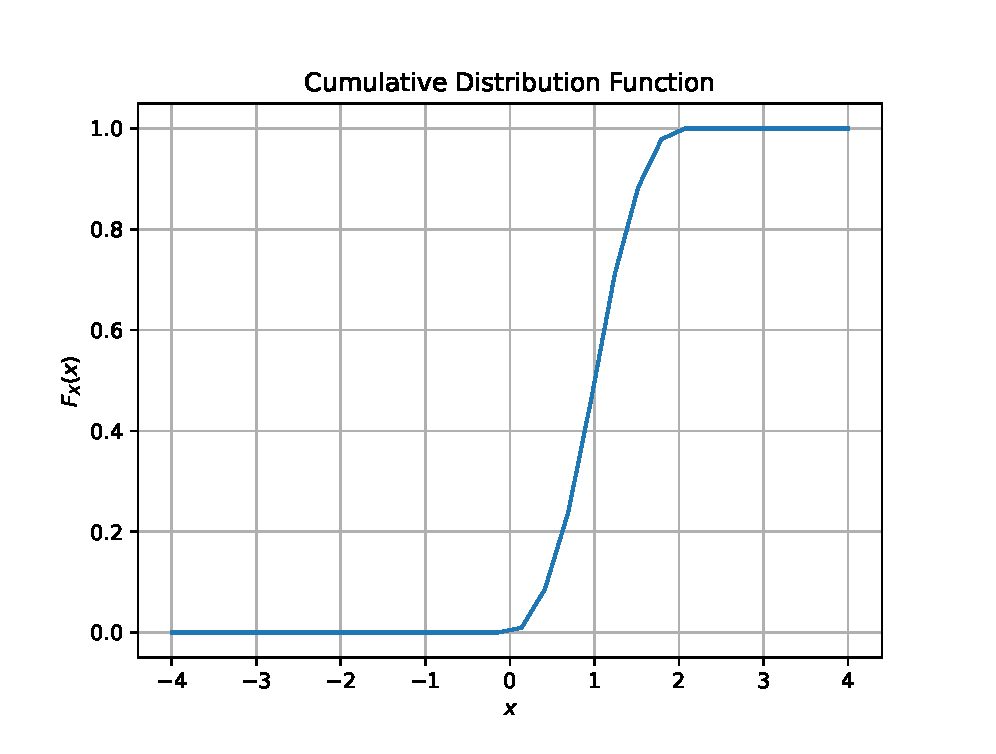
\includegraphics[width=\columnwidth]{./figs/t_cdf}
\caption{The CDF of $T$}
\label{fig:t_cdf}
\end{figure}
\item Find the PDF of $T$.\\
\solution
The code for the PDF of T is in
\begin{lstlisting}
Assignment 4/codes/pdf_plot.py
\end{lstlisting}
\begin{figure}
\centering
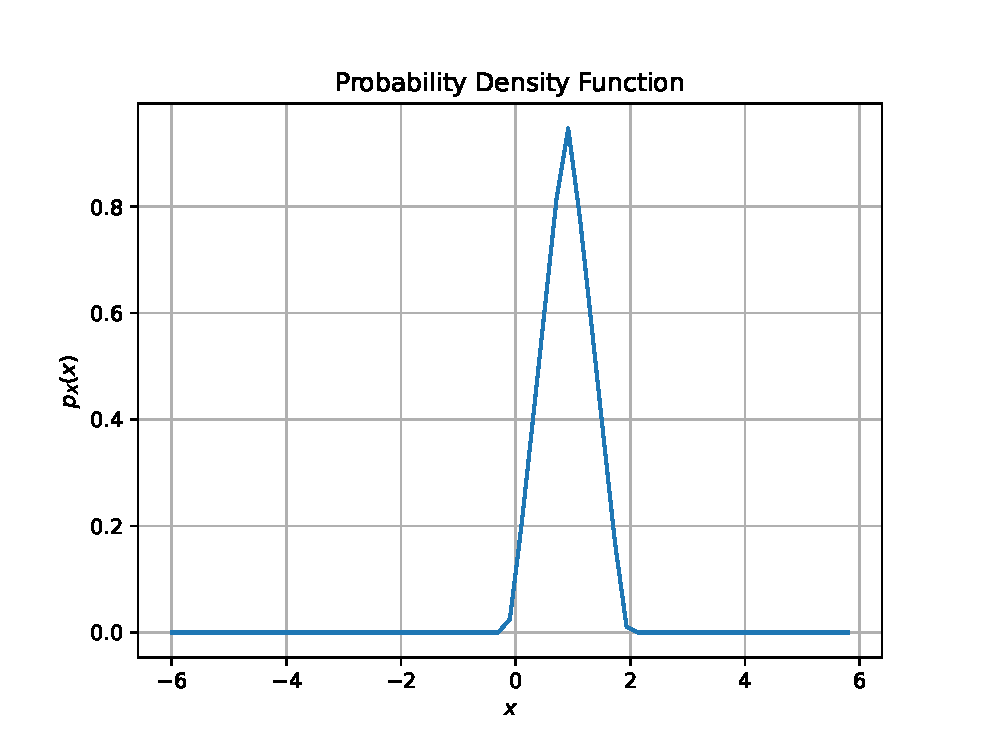
\includegraphics[width=\columnwidth]{./figs/t_pdf}
\caption{The PDF of $T$}
\label{fig:t_pdf}
\end{figure}
\item Find the theoretical expressions for the PDF and CDF of $T$.\\
\solution
We know that if $X$ and $Y$ are independent distributions, then we  can use convolution formula for getting the PDF of $F_{X+Y}$ as 
\begin{equation}
f_{X+Y}(t)=\int_{\infty}^{\infty} f_X(x)f_Y(t-x)dx
\end{equation}
And the CDF of $F_{X+Y}$ is given as
\begin{equation}
F_{X+Y}(t)=\int_{-\infty}^t f_{X+Y}(x)dx
\end{equation}
Accordingly, for our casee $U_1$ and $U_2$ are uniform i.i.d. random variables in [0, 1]. Then, $0 \leq U_1 + U_2 \leq 2$.
Again we know that 
\begin{align*}
f_{U_1}(x)=
	 \begin{cases}
    0 & \text{for x $<$ 0}\\
      1 & \text{for x $\geq$ 0}
    \end{cases}
     \\    
F_{U_1}(x)=\pr{U_1 \le x} =
    \begin{cases}
    0 & \text{for x $<$ 0}\\
      x & \text{for}~x\in [0,1]\\
      1 & \text{for x $>$ 1}
    \end{cases}       
\end{align*} and 
\begin{align*}
f_{U_2}(x)=
	 \begin{cases}
    0 & \text{for x $<$ 0}\\
      1 & \text{for x $\geq$ 0}
    \end{cases}
     \\
  F_{U_2}(x)=\pr{U_2 \le x} =
    \begin{cases}
    0 & \text{for x $<$ 0}\\
      x & \text{for}~x\in [0,1]\\
      1 & \text{for x $>$ 1}
    \end{cases}  
\end{align*}
Now we deal with the interval from 0 to 2. It is useful to break this down into two cases (i) $0\leq t< 1$ and (ii) $1\leq t <2$.\\ \\
Case (i): $0\leq t<1$. The product $f_{U_1}(x)f_{U_2}(t-x)$ is 1 in someplaces and 0 elsewhere. So, for $f_{U_2}(t-x)=1$ we need $t-x\geq 0$ and thus $x\leq t$ and therefore, we integrate from $x=0$ and $x=t$. 
\begin{align*}
f_{T}(t)&=\int_{0}^{t} 1.1 dt=t
\\
F_T(t)&=\int_{0}^{t} f_{T}(t)dt
\\
&=\int_{0}^{t} t dt
\\
&=\frac{t^2}{2}
\end{align*}
Case (ii): For $1\leq t <2$, Again for $f_{U_2}(t-x)=1$ we need $t-x\leq 1$ and thus $x\leq t-1$ and therefore, we integrate from $x=t-1$ and $x=1$. 
\begin{align*}
f_{T}(t)&=\int_{t-1}^{1} 1.1 dx
\\
&=\left[t\right]_{t-1}^{1}=2-t
\\
F_T(t)&=\int_{0}^{t} f_{T}(t)dt
\\
&=\int_{0}^{1} tdt +\int_{1}^{t} (2-t)dt 
\\
&=\left[\frac{t^2}{2}\right]_0^1+\left[2t-\frac{t^2}{2}\right]_1^t
\\
&=2t-\frac{t^2}{2}-1
\end{align*}
So, the CDF for T is given by 
\begin{equation}
F_{T}(t)=\pr{T \le t} =
    \begin{cases}
    0 &  x< 0\\
      \frac{t^2}{2} & 0\leq t<1\\
      2t-\frac{t^2}{2}-1 & 1\leq t<2\\
      1 & x\geq 2
    \end{cases}  
\end{equation}
and the PDF for T is given by 
\begin{equation}
f_{T}(t)=
	 \begin{cases}
    t & 0\leq t<1\\
    2-t & 1\leq t<2\\
    0 & \text{Elsewhere}  
    \end{cases}
\end{equation}
\item Verify your results through a plot. \\
\solution
The Figures \ref{fig:t_cdf} and \ref{fig:t_pdf} suffice the purpose.
\end{enumerate}

\end{document}

